\def\QRCODE{TB_image_TUT.IMG.image_restoration_deblurring_matlabqrcode.png}
\def\QRPAGE{http://www.iptutorials.science/tree/master/TB_image/TUT.IMG.image_restoration_deblurring/matlab}
\mcorrectionsection{Matlab correction}

\subsection{Damage modeling}

The damaged image is generated using the following method, illustrated in Fig. \ref{fig:deblurring:matlab:noisy}, for a motion perturbation. Notice the \minline{'circular'} option in the convolution, which acts as if the psf would be periodic (this is the case in the Fourier space).

\begin{matlab}
% generates a noisy image, with motion blur
f = checkerboard(8);
psf = fspecial('motion',7,45);
gb = imfilter(f,psf,'circular');
noise = imnoise(zeros(size(f)),'gaussian',0,0.001);
g = gb + noise;
\end{matlab}

The noise can also be generated by the following command:
\begin{matlab}
sigma = .1;
noise = randn(size(f)) * sigma;
\end{matlab}

\begin{figure}[htbp]
 \centering
 \subfloat[Original image.]{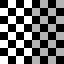
\includegraphics[width=.3\linewidth]{original_image.png}}\hspace{1cm}
 \subfloat[Movement blur.]{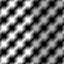
\includegraphics[width=.3\linewidth]{movement.png}}
 
 \subfloat[Gaussian noise.]{
\includegraphics[width=.3\linewidth]{noise.png}}\hspace{1cm}
 \subfloat[Noisy image.]{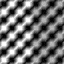
\includegraphics[width=.3\linewidth]{degraded.png}}
 
 \caption{Simulation of damaged images.\label{fig:deblurring:matlab:noisy}}
 
\end{figure}

If the psf used is gaussian, the command will be:
\begin{matlab}
psf = fspecial('gaussian', size(f), 1);
\end{matlab}


\subsection{Inverse filtering with no noise}

\begin{mcomment}
\begin{mremark}
Be careful to use \minline{psf2otf} instead of \minline{fft2}. This is basically the same purpose, but the latter lacks centering when performing the array padding.
\end{mremark}
\end{mcomment}

The inverse filter of the damaged image is performed using the following \matlabregistered{} command. 
The result is illustrated in Fig. \ref{fig:deblurring:matlab:nonoise}.

\begin{matlab}
% Fourier Transform of the psf
H = psf2otf(psf, size(f));
G = fft2(g);

% pseudo inverse: ensures there is no division by 0
alpha = 0.01;
F = G./(H + alpha);
fr= ifft2(F);
\end{matlab}

\begin{figure}[htbp]
 \centering
 \subfloat[Pseudo inverse filter, $\alpha=0.1$.]{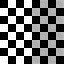
\includegraphics[width=.3\linewidth]{pseudo_inverse.png}}\hspace{1cm}
 \subfloat[Wiener filter.]{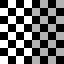
\includegraphics[width=.3\linewidth]{wiener_motion_nonoise.png}}
 \caption{Motion blur, 45 degrees, with no noise.}
 \label{fig:deblurring:matlab:nonoise}
\end{figure}

\subsection{Wiener filter}
\subsubsection{Simple case: no noise}
\begin{matlab}
% Fourier Transform of the psf
H = psf2otf(psf, size(f));
G = fft2(g);

% Wiener filter when no noise
% Eliminates zeros values in H
H(H==0) = Inf;
F = G./H;
fw = ifft2(F);
\end{matlab}
The result is illustrated in Fig.\ref{fig:deblurring:matlab:nonoise}

\subsubsection{Noisy images}
To evaluate the ratio $R$, the following commands are performed:
\begin{matlab}
SpecPuissNoise=abs(fft2(noise)).^2;
PuissMoyNoise=sum(SpecPuissNoise(:))/numel(noise);
SpecPuissImageOrig=abs(fft2(f)).^2;
PuissMoyImageOrig=sum(SpecPuissImageOrig(:))/numel(f);
ratio=PuissMoyNoise/PuissMoyImageOrig;
\end{matlab}

And then, the Wiener filter is applied either as a \matlabregistered{} function or as your own function. The result of this second version is presented in Fig. \ref{fig:deblurring:matlab:wienernoise}.

\begin{matlab}
% \matlabregistered{} function
fr2=deconvwnr(g,psf,ratio);
\end{matlab}

\begin{matlab}
% create a damaged image with some noise
f=checkerboard(8);
psf = fspecial('gaussian', size(f), 2);
% noise
sigma=.01; 
N = randn(size(f)) * sigma;
g = imfilter(f, psf, 'circular') + N;
g = max(0,g);
g = min(1,g);

% performs the restoration
H = psf2otf(psf, size(f)); % Fourier Transform of the psf
Hw = conj(H)./(abs(H).^2+PuissMoyNoise/PuissMoyImageOrig);
fr = ifft2( Hw .* fft2(g));
\end{matlab}

\begin{figure}
 \centering
 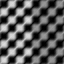
\includegraphics[width=5cm]{wiener_motion_noise.png}
 \caption{Wiener filter with approximated ratio $R$.}
 \label{fig:deblurring:matlab:wienernoise}
\end{figure}

\newpage
\subsection{Iterative filters for noisy images}
\subsubsection{Van Cittert iterative filter}
The VanCittert algorithm is maybe the simplest iterative method. It is really sensitive to noise, as illustrated in Fig. \ref{fig:deblurring:matlab:vancittert_motion_10}.

\begin{figure}[htbp]
 \centering
 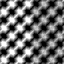
\includegraphics[width=5cm]{vancittert_motion_10.png}
 \caption{VanCittert iterative restoration algorithm with 10 iterations, applied on an image damaged with motion blur and gaussian white noise. This algorithm is really sensitive to noise.}
 \label{fig:deblurring:matlab:vancittert_motion_10}
\end{figure}

\begin{matlab}
function [ fr ] = vca( g, psf, n_iter)
% Van Cittert iteration algorithm for deconvolution
%
% g: degraded image
% psf: point spread function
% n_iter: number of iterations

% Fourier Transform of the psf
H = psf2otf(psf, size(g));

% initialization
fr=g;

beta = .1; % Jansson parameter
for iter = 1:n_iter
    fr = fr + beta*(g -ifft2(H .* fft2(fr)));
end

end
\end{matlab}

\subsubsection{Lucy-Richardson filtering}

The Lucy-Richardson deconvolution filter is one of the most employed filter. The convolution operations can be either performed in the Fourier (frequency) domain, or in the spatial domain. For performance reasons, it is usually better to work in the Fourier domain, where the convolution is transform into a simple product. The results are presented in Fig. \ref{fig:deblurring:matlab:lucy_motion}

\begin{matlab}
function fr = rla(g, psf, n_iter)
% Richardson-Lucy Algorithm for deconvolution
%
% g: image to restore. initial value of fr is g
% psf: point spread function
% n_iter: number of iterations

% Optical Transfer Function
H = psf2otf(psf, size(g));

% initial value
fr = g;

% iterations
for iter=0:n_iter
    % estimated blurred image
    yk = (ifft2(H.*fft2(fr)));
    
    M = ifft2(conj(H) .* fft2(g./yk));
    fr = max(0,fr.* M);
end
\end{matlab}

\begin{figure}[htbp]
 \centering
 
 \subfloat[Algorithm with 100 iterations.]{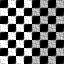
\includegraphics[width=.3\linewidth]{rla_motion_100.png}}
 \hspace{1cm}
 \subfloat[Algorithm with 10 iterations.]{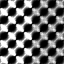
\includegraphics[width=.3\linewidth]{rla_motion_10.png}}
 
 \caption{Lucy-Richardson algorithm applied on the chessboard image with motion blur and gaussian white noise.}
 \label{fig:deblurring:matlab:lucy_motion}
\end{figure}

\newpage
\subsection{Blind deconvolution}
The first step is to generate a degraded image, as before.
\begin{matlab}
f=checkerboard(8);
S = 10; % size of PSF
psf=fspecial('gaussian',S,10);
sd=0.01; % std deviation of the generated noise

% add some gaussian noise with 0 mean and variance sd^2
g=imnoise(imfilter(f,psf, 'circular'),'gaussian', 0, sd^2);
\end{matlab}

The \minline{dampar} variable is a damping parameter to minimize the noise (see \matlabregistered{} help).

\begin{matlab}
% damping parameter
dampar=10*sd;

% create initial psf
initpsf=ones(S);

% apply blind deconvolution for nb_iterations
nb_iterations = 5;
[fr_blind, psfe]=deconvblind(g,initpsf, nb_iterations, dampar);
\end{matlab}

\begin{figure}[htbp]
\centering
\subfloat[Original image.]{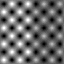
\includegraphics[width=5cm]{deconvblind_originale.png}}

\subfloat[Blind deconvolution for 100 iterations.]{
\includegraphics[width=5cm]{BD_100.png}}
\hspace{1cm}
\subfloat[Blind deconvolution for 5 iterations.]{
\includegraphics[width=5cm]{BD_5.png}}

\subfloat[PSF used for image degradation.]{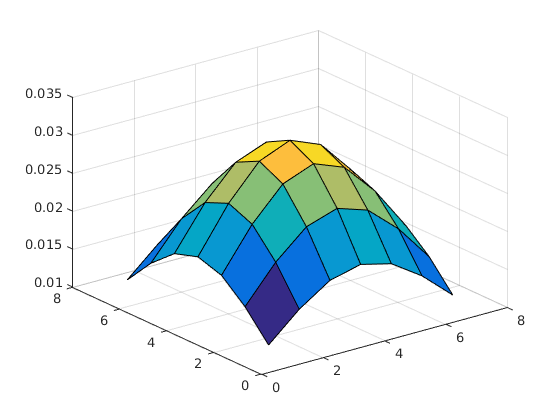
\includegraphics[width=5cm]{psf.png}}
\hspace{1cm}
\subfloat[PSF estimated after blind deconvolution.]{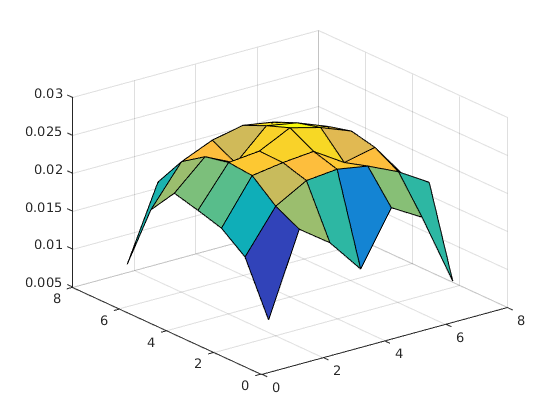
\includegraphics[width=5cm]{deconvblind_psfe.png}}

 \caption{Blind deconvolution}
 \label{fig:deblurring:matlab:blind}
\end{figure}

\begin{figure}[htbp]
 \centering
 
 \subfloat[Original image of Jupiter.]{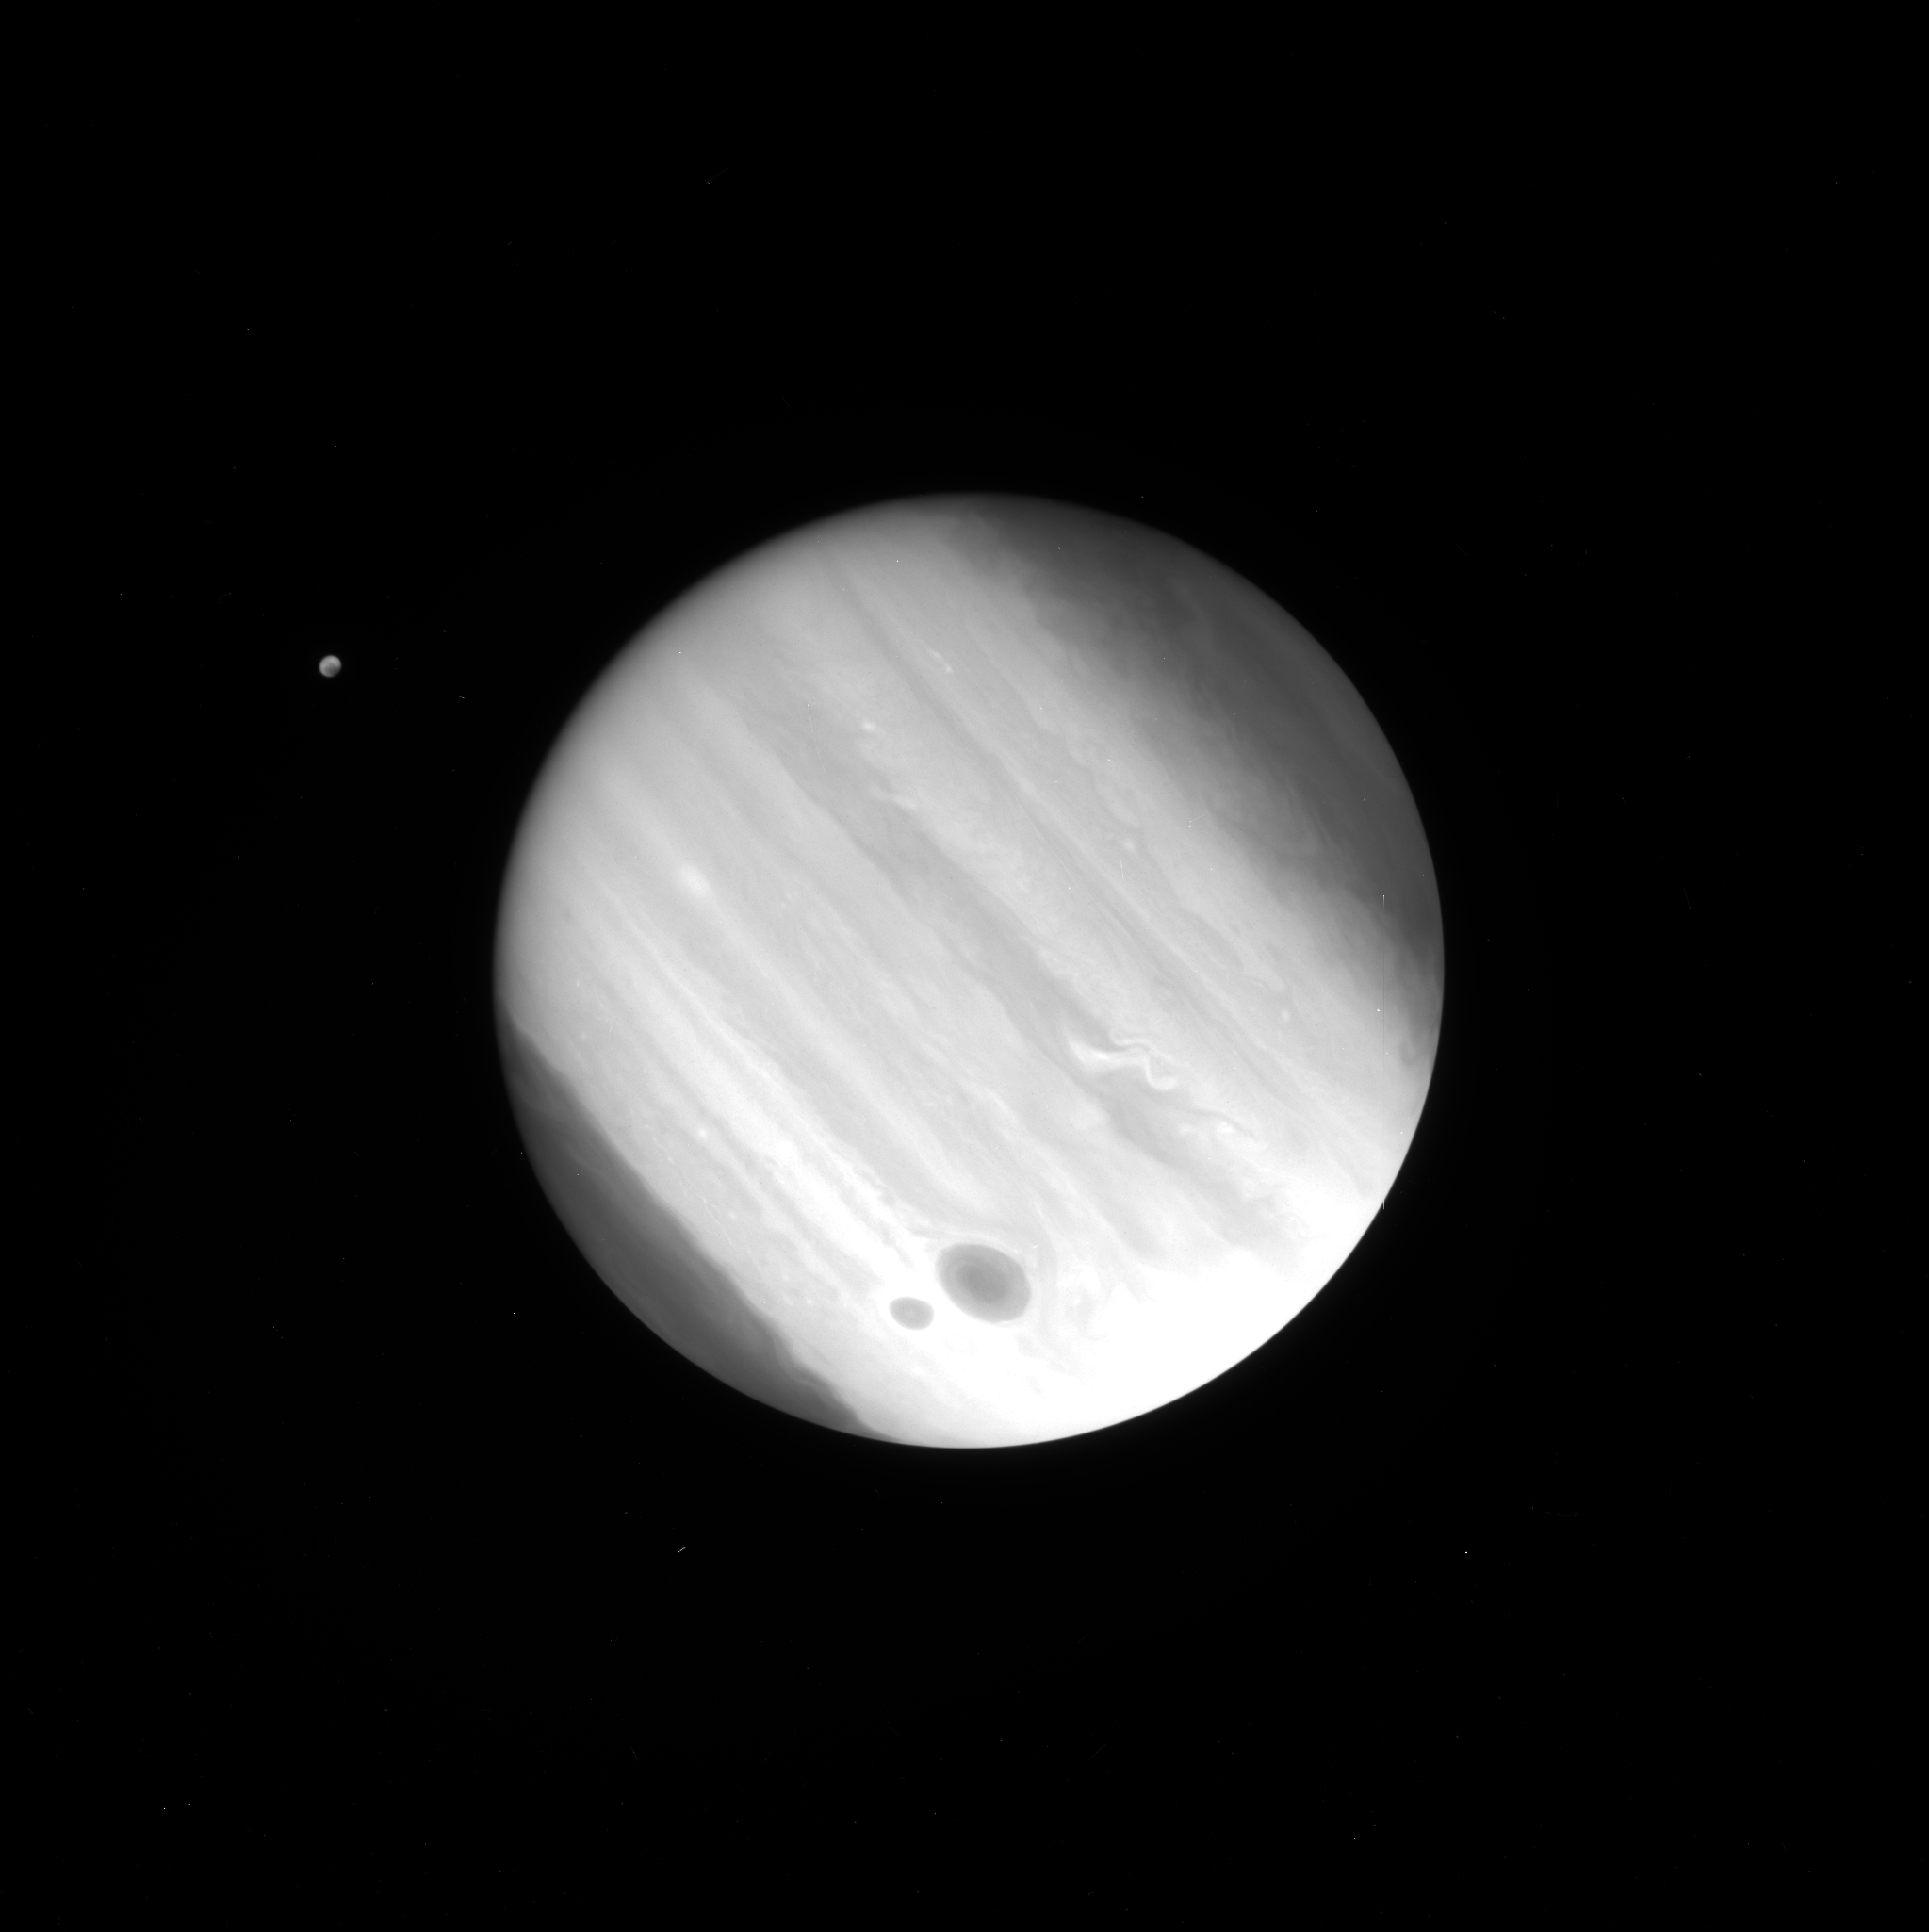
\includegraphics[width=7cm]{original_jupiter.png}}
 
 \subfloat[Jupiter image after Lucy-Richardson algorithm with 10 iterations.]{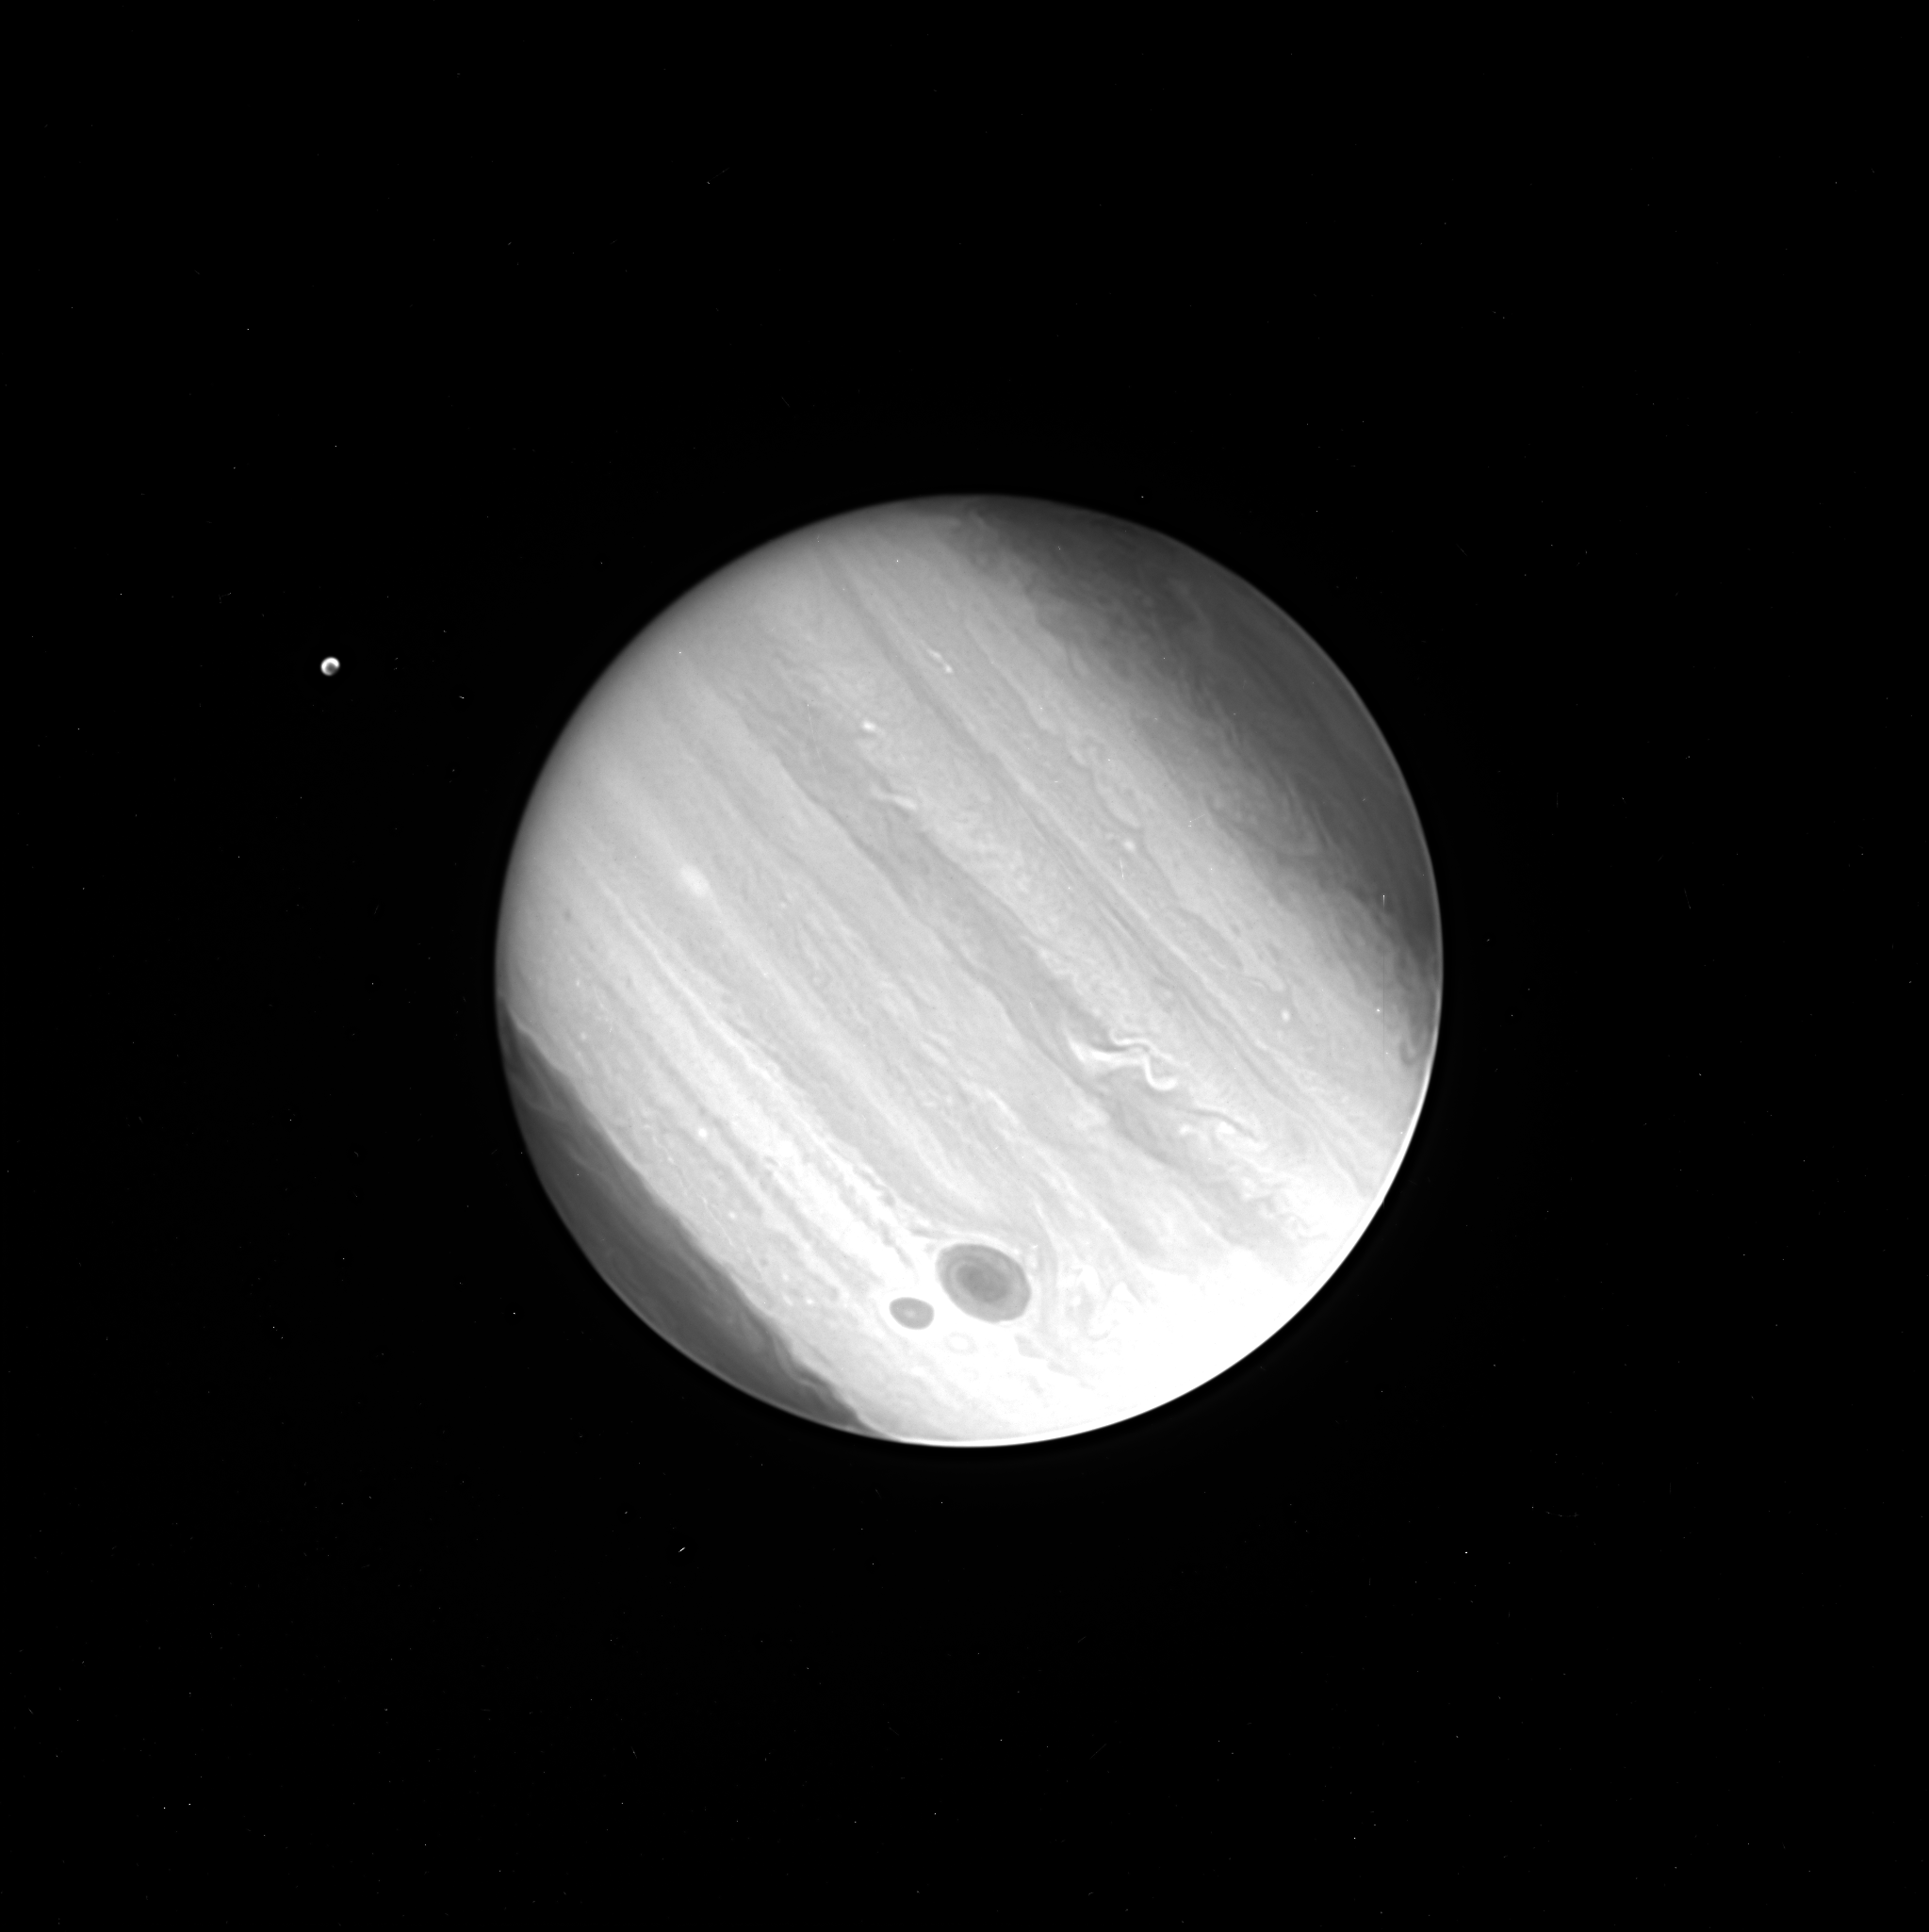
\includegraphics[width=7cm]{rla_jupiter.png}}
 \caption{Jupiter, from Hubble Space Telescope, ads/Sa.HST\#ic3g01qlq.}
\end{figure}

\begin{figure}[htbp]
 \centering
 
 \subfloat[Original image of Saturn.]{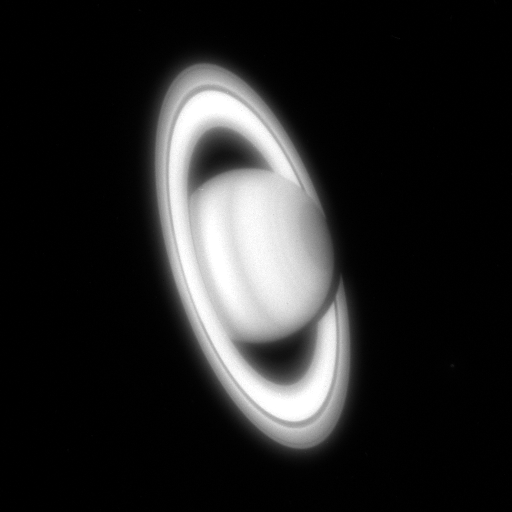
\includegraphics[width=7cm]{original_saturn.png}}
 
 \subfloat[Saturn image after Lucy-Richardson algorithm with 100 iterations.]{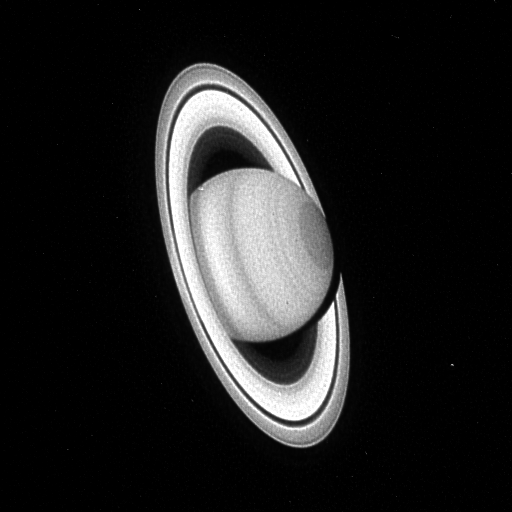
\includegraphics[width=7cm]{rla_saturn.png}}
 \caption{Saturn, from Hubble Space Telescope.}
\end{figure}